\chapter{Zadatak A} \label{ch:a}
U ovom poglavlju je opisan i odrađen zadatak A.

\section{Opis zadatka} \label{sec:a:opis}
Prikazati krivulje kretanja u 2D i 3D obliku, krivulje prijeđenog puta [u SI jeidnicama], brzine vožnje[u
SI jeidnicama], ubrzanja[u SI jeidnicama], promjene visine[u SI jeidnicama], nagiba ceste [u
jedinicama : rad, °, \%]. Dodatno, za svaku varijablu je potrebno odrediti minimalnu, maksimalnu i
srednju vrijednost krivulje, te prikazati je u tabličnom obliku.
Napomena a) : potrebno je prikazati “čitljive“ podatke, to upućuje na korištenje filtera (kao
„movAvgFilt“) u svrhu izglađivanja krivulje, ali uz to da se ne izgubi stvarna slika krivulje. Potrebno
je filtrirati većim intezitetom i eventualno ograničit promjenu visine na način da nagib ceste ne
prelazi vrijednost od ±10\%.

\section{Rješenje} \label{sec:a:rjesenje} Zadatak je riješenje koristeći Python
i biblioteke \textit{NumPy}, \textit{MatPlotLib} i \textit{Polars}. U nastavku je opisan postupak
rješavanja zadatka.

Prije svega, potrebno je učitati podatke iz datoteke \textit{data.csv}. To je
napravljeno pomoću funkcije \textit{read\_csv} koja vraća \textit{DataFrame} objekt koji
sadrži sve podatke iz datoteke. Nakon toga bilo je potrebno pretvoriti tipove
podataka u \textit{float} kako bi se mogli koristiti u daljnjem radu. Izračunat je i
stupac \textit{DateTime} koji sadrži vrijeme u obliku \textit{DateTime}. Nakon toga,
potrebno je izbaciti stršeće vrijednosti iz podataka. Na kraju su nacrtani
svi traženi grafovi koristeći \textit{MatPlotLib}.

\begin{figure}
    \centering
    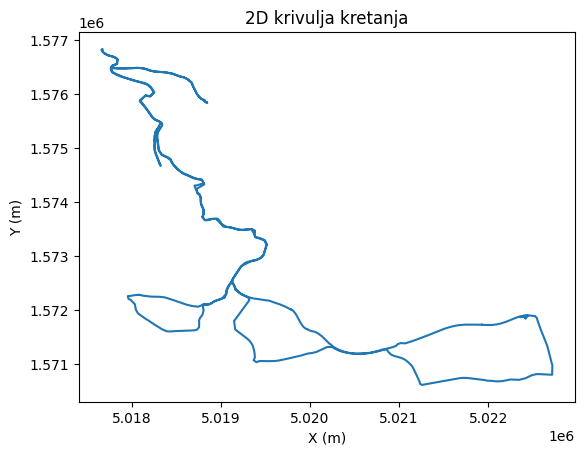
\includegraphics[width=0.8\textwidth]{images/path_2d.png}
    \caption{2D prikaz krivulje kretanja.}
    \label{fig:a:2d}
\end{figure}

\begin{figure}
    \centering
    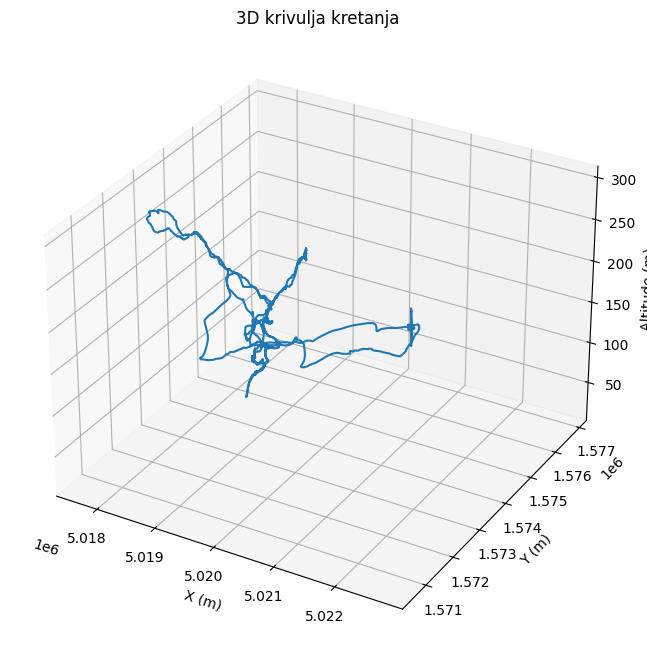
\includegraphics[width=0.8\textwidth]{images/path_3d.png}
    \caption{3D prikaz krivulje kretanja.}
    \label{fig:a:3d}
\end{figure}

\begin{figure}
    \centering
    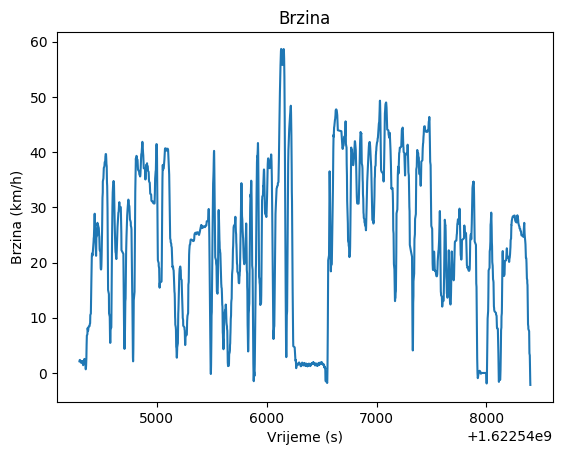
\includegraphics[width=0.8\textwidth]{images/speed.png}
    \caption{Prikaz izmjerene brzine kretanja kroz vrijeme.}
    \label{fig:a:speed}
\end{figure}

\begin{figure}
    \centering
    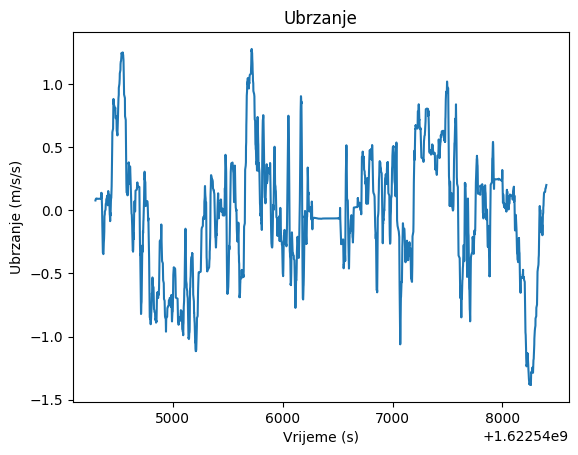
\includegraphics[width=0.8\textwidth]{images/acceleration.png}
    \caption{Prikaz izmjerenog ubrzanja kretanja kroz vrijeme.}
    \label{fig:a:acceleration}
\end{figure}

\begin{figure}
    \centering
    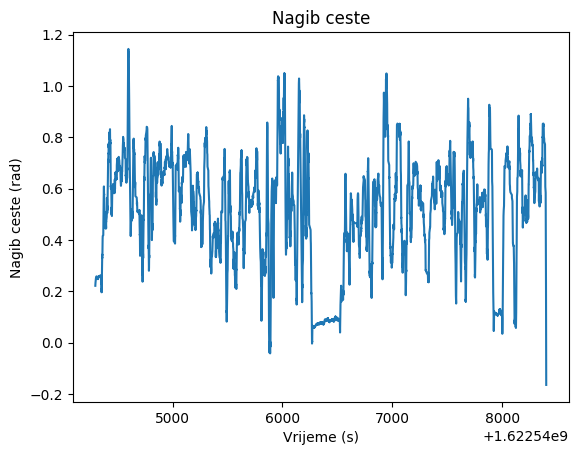
\includegraphics[width=0.8\textwidth]{images/road_angle.png}
    \caption{Prikaz izmjerenog nagiba ceste kroz vrijeme.}
    \label{fig:a:road_angle}
\end{figure}

\begin{figure}
    \centering
    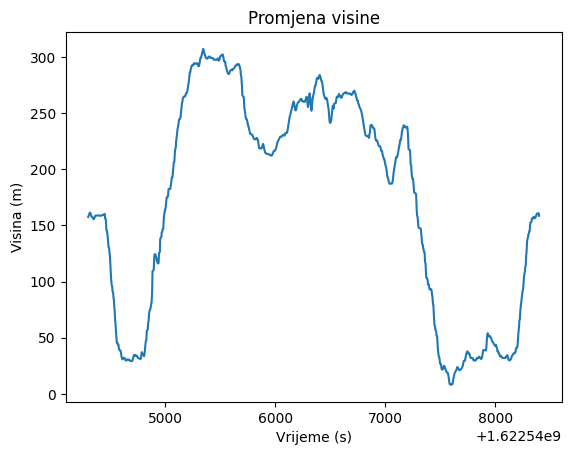
\includegraphics[width=0.8\textwidth]{images/height.png}
    \caption{Prikaz izmjerene nadmorske visine kroz vrijeme.}
    \label{fig:a:height}
\end{figure}

\begin{figure}
    \centering
    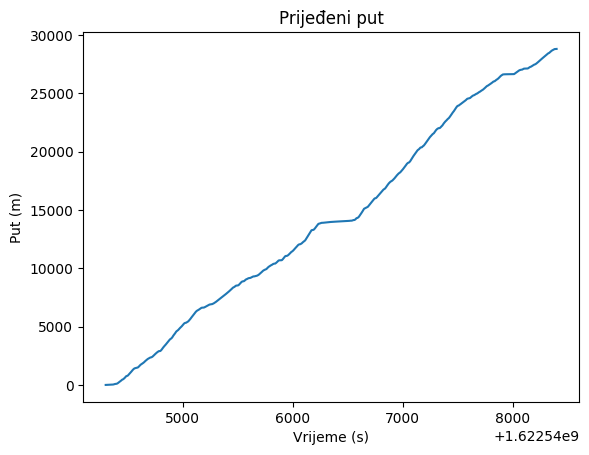
\includegraphics[width=0.8\textwidth]{images/traveled.png}
    \caption{Prikaz izračunatog prijeđenog puta kroz vrijeme.}
    \label{fig:a:distance}
\end{figure}


\begin{table}[!ht]
    \centering
    \caption{Opis podataka.}
    \begin{tabular}{lllll}
    \hline
        \textbf{describe} & \textbf{AccelerationX} & \textbf{AccelerationY} & \textbf{AccelerationZ} & \textbf{GyroscopeX} \\ \hline
        count & 9776.0 & 9776.0 & 9776.0 & 9776.0 \\ 
        null\_count & 0.0 & 0.0 & 0.0 & 0.0 \\ 
        mean & -0.050049 & -0.004825 & 1.003017 & -0.440136 \\ 
        std & 0.037009 & 0.058152 & 0.010231 & 0.53678 \\ 
        min & -0.17733 & -0.17736 & 0.97196 & -2.08956 \\ 
        25\% & -0.07448 & -0.03706 & 0.99773 & -0.68926 \\ 
        50\% & -0.0427 & -0.00652 & 1.00438 & -0.45114 \\ 
        75\% & -0.03152 & 0.0284 & 1.00763 & -0.20376 \\ 
        max & 0.06896 & 0.17369 & 1.03259 & 1.21343 \\ \hline
    \end{tabular}
    \label{table:a:data}
\end{table}

\begin{table}[!ht]
    \centering
    \caption{Opis podataka.}
    \begin{tabular}{llllll}
    \hline
        \textbf{GyroscopeY} & \textbf{GyroscopeZ} & \textbf{Latitude} & \textbf{Longitude} & \textbf{Velocity} & \textbf{Altitude} \\ \hline
        9776.0 & 9776.0 & 9776.0 & 9776.0 & 9776.0 & 9776.0 \\ 
        0.0 & 0.0 & 0.0 & 0.0 & 0.0 & 0.0 \\ 
        -0.004038 & 0.052931 & 14.134695 & 45.092696 & 22.580305 & 174.023895 \\ 
        0.558823 & 1.41705 & 0.018312 & 0.014516 & 15.827058 & 97.517645 \\ 
        -1.66491 & -4.23632 & 14.109408 & 45.075358 & 0.0 & 6.4 \\ 
        -0.24799 & -0.39591 & 14.12051 & 45.080807 & 2.5928 & 51.2 \\ 
        0.00122 & -0.06167 & 14.12425 & 45.086985 & 25.5576 & 215.1 \\ 
        0.24188 & 0.49669 & 14.155648 & 45.103833 & 35.7436 & 258.1 \\ 
        1.66778 & 4.25036 & 14.165298 & 45.120837 & 59.6344 & 308.8 \\ \hline
    \end{tabular}
    \label{table:a:data2}
\end{table}

\begin{table}[!ht]
    \centering
    \caption{Opis podataka.}
    \begin{tabular}{llll}
    \hline
        \textbf{Position} & \textbf{DateTime} & \textbf{Y} & \textbf{X} \\ \hline
        9776.0 & """9776""" & 9776.0 & 9776.0 \\ 
        0.0 & """0""" & 0.0 & 0.0 \\ 
        10.795417 & null & 1.5734e6 & 5.0196e6 \\ 
        0.403417  & null & 2038.45233 & 1615.866881 \\ 
        10.0  & """2021-06-01 10:44:57.688000""" & 1.5706e6 & 5.0177e6 \\ 
        11.0 & null & 1.5719e6 & 5.0183e6 \\ 
        11.0 & null & 1.5723e6 & 5.0190e6 \\ 
        11.0  & null & 1.5758e6 & 5.0208e6 \\ 
        11.0  & """2021-06-01 11:53:18.980000""" & 1.5768e6 & 5.0227e6 \\ \hline
    \end{tabular}
    \label{table:a:data3}
\end{table}







